\begin{figure*}[!h]
    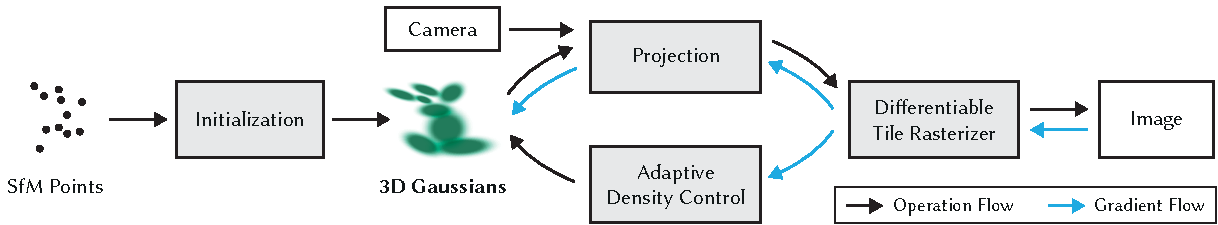
\includegraphics[width=\linewidth]{figures/overview/overview_01.pdf}
    \caption{
        Оптимизация начинается с разреженного облака точек SfM и создает набор 3D Гауссиан. Затем мы оптимизируем и адаптивно контролируем плотность этого набора Гауссиан. Во время оптимизации мы используем наш быстрый растеризатор на основе тайлов, что позволяет достичь конкурентного времени обучения по сравнению с самыми быстрыми современными методами радиусных полей. После обучения наш рендерер обеспечивает навигацию в реальном времени для широкого спектра сцен.
    }
    \label{fig:overview}
\end{figure*}
\section{Обзор}
Входными данными для нашего метода являются изображения статической сцены вместе с соответствующими камерами, откалиброванными с помощью SfM \cite{schoenberger2016sfm}, который в качестве побочного эффекта создает разреженное облако точек.
Из этих точек мы создаем набор 3D Гауссиан %
(Раздел~\ref{sec:3d-splats}), 
определяемых позицией (средним значением), матрицей ковариации и непрозрачностью $\alpha$, что позволяет использовать очень гибкий режим оптимизации. В результате получается достаточно компактное представление 3D сцены, отчасти потому, что высокоанизотропные объемные сплаты могут компактно представлять мелкие структуры. Направленная составляющая внешнего вида (цвет) радиусного поля представляется с помощью сферических гармоник (SH), что является стандартной практикой~\cite{plenoxels,mueller2022instant}. Наш алгоритм переходит к созданию представления радиусного поля (Раздел~\ref{sec:opt-dens}) через последовательность шагов оптимизации параметров 3D Гауссиан, то есть положения, ковариации, $\alpha$ и коэффициентов SH, чередующихся с операциями для адаптивного контроля плотности Гауссиан.
Ключом к эффективности нашего метода является наш растеризатор на основе тайлов (Раздел~\ref{sec:tile-raster}), который позволяет выполнять $\alpha$-смешивание анизотропных сплатов, учитывая порядок видимости благодаря быстрой сортировке. Наш быстрый растеризатор также включает быстрый обратный проход, отслеживая накопленные значения $\alpha$, без ограничения на количество Гауссиан, которые могут получать градиенты.
Обзор нашего метода представлен на Рис.~\ref{fig:overview}.